\documentclass{article}
\usepackage[utf8]{inputenc}
\usepackage[francais]{babel}
\usepackage{lmodern}
\usepackage[a4paper, margin=3cm]{geometry}
\usepackage{fancyhdr}

%Package for math expression
\usepackage{amsmath}
\usepackage{cancel}
\usepackage{amsthm,amstext,amsfonts,bm,amssymb,amsthm}
\usepackage{bm}
\usepackage{gensymb}
\usepackage{mathrsfs}
\usepackage{physics}
\usepackage{nicefrac}
\usepackage{pgffor}

%Package for graphic expression
\usepackage{graphicx}
\usepackage{wrapfig}
\usepackage{float}
\usepackage{caption}
\usepackage{subcaption}
\usepackage{enumitem}
\usepackage{fancyhdr}
\usepackage{sectsty}
\usepackage{multirow}

\usepackage{mathtools}
\DeclarePairedDelimiter\ceil{\lceil}{\rceil}
\DeclarePairedDelimiter\floor{\lfloor}{\rfloor}

\usepackage{pgffor}

\DeclarePairedDelimiter\absol{\lvert}{\rvert}%

% Header
\pagestyle{fancy}
\fancyhf{}
\rhead{Éric Pfleiderer}
\fancyhead[L]{À la recherche du boson de Higgs}
\chead{}
\rfoot{}
\cfoot{\thepage}

\begin{document}
	
\begin{titlepage}
	\centering
	\vspace*{1cm}
	\textsc{\LARGE Université de Montréal}\\[1cm] 
	\textsc{\Large PHY 3075 -- Modélisation Numérique en Physique}\\[3cm]
	\vspace{1cm}
	\rule{\linewidth}{0.5mm} \\[0.5cm]
	{\LARGE \bfseries À la recherche du boson de Higgs} \\[0.2cm]
	\rule{\linewidth}{0.5mm} \\[3cm]
	\vspace{1cm}
	\large par: \\*
	Éric Pfleiderer \\* 
	20048976\\[3cm] 
	\vspace{1cm}
	{\large \today}\\[3cm]
	\vfill
\end{titlepage}


\section*{Résumé}

\begin{center}
	L'objectif de ce laboratoire est de développer un modèle d'apprentissage machine pour solutionner un problème de classification binaire: la recherche du boson de Higgs. À cette fin, on emploie les librairies Tensorflow et Keras, qui fournissent une variété de fonctions de perte, d'optimiseurs, de fonctions d'activation et d'architectures. Afin d'augmenter la performance de notre modèle, on compare la performance des optimiseurs, on détermine le rythme d'apprentissage approprié au problème et on analyse les statistiques d'erreur. On trouve que la performance des optimiseurs est similaire, sauf pour la descente stochastique du gradient. Le rythme d'entraînement optimal, quant à lui, se situe entre $1\times10^{-5}$ et $2\times10^{-4}$. La performance de classification moyenne obtenue est de $82.44\%$, avec un léger biais pour les vrai positifs.
\end{center}

\section{Description du réseau}

Depuis le déploiement de ses dernières versions, la librairie d'apprentissage machine Tensorflow\cite{tensorflow} intègre l'interface de programmation Keras\cite{keras}, qui facilite le déploiement et l'entraînement de réseaux neuronaux. Dans le cadre de ce laboratoire, on explore Keras à la recherche d'un modèle et d'une technique d'optimisation. On considère l'architecture et les fonctions d'activations du modèle, ainsi que la fonction de perte et l'optimiseur employés durant l'entraînement. L'architecture du modèle est définit par ses hyperparamètres, soit le nombre et le type de couches, ainsi que le nombre de neurones par couche. L'implémentation du réseau est disponible sur le dépot  GitHub de l'auteur \cite{github}.

\subsection{Fonctions de perte}

Keras offre plusieurs méthodes de classification d'erreur qui sont plus ou moins efficaces dépendemment de la situation. Parmi ces méthodes, on compte entre autres les erreurs absolues, les erreurs quadratiques, ainsi que des types d'erreur plus particuliers comme le logcosh et l'entropie croisée. Dans le cas de la classification binaire, une fonction de perte populaire est l'entropie croisée, donnée par l'équation \ref{eq:loss}, où $y$ est la réponse désirée et $p$ est la prédiction. Cette fonction de perte peut être généralisée pour tout autre problème de classification.

\begin{equation}\label{eq:loss}
	E_{cr} = -y\ log(p) + (1-y)\ log(1-p)
\end{equation}

\subsection{Optimiseurs}

Keras offre aussi une multitude d'optimiseurs, du plus traditionel, tel que la descent stochastique du gradiant,  au plus sophistiqué, tel que Adadelta, qui modifie le rythme d'apprentissage selon les dernières mises à jour du gradient. Puisqu'on ne peut prédire quel optimiseur est approprié pour le problème de classification du boson de Higgs, on compare leur performance à partir de la même solution initiale. Additionnellement, on doit aussi trouver le rythme d'apprentissage approprié. Ces analyses, ainsi que leur résultat, sont présentées à la section \ref{sec:stat_err}.

\subsection{Fonctions d'activation}

Le choix des fonctions d'activation est relativement simple. Puisque la sortie du réseau doit représenter une probabilité, on doit écraser le signal arrivant à la dernière couche entre 0 et 1. La fonction sigmoïd est idéale pour accomplir cette tâche. Ensuite, on choisit la fonction de type relu comme fonction d'activation pour le reste des couches. Cette fonction d'activation empêche la saturation du gradient, ce qui tend a accélérer la convergence de certains optimiseurs comparativement aux fonctions sigmoïd et tanh.

\subsection{Architecture et hyperparamètres}

On doit maintenant choisir les hyperparamètres de notre réseau neuronal. Un réseau peu profond avec une faible quantité de neurones par couche ne parviendra pas a généraliser son apprentissage et ne pourra prédire qu'une faible fraction de l'ensemble de données (underfitting). Inversément, si le réseau devient trop profond et trop large, l'optimisation peut alors se traduire par une mémorisation de l'ensemble de donnée (overfitting). L'optimisation tend alors a diminuer la performance de prédiction du réseau sur l'ensemble de test. L'architecture choisie est affichée et décrite à la figure \ref{fig:model} en annexe.

\section{Statistiques d'erreur}\label{sec:stat_err}

Dans cette section, on s'intéresse à analyser les statistiques d'erreur lors de l'entraînement et de la validation afin d'appuyer la crédibilité de nos classifications. On s'intéresse initialement aux statistiques d'entraînement, où on compare la performance des différents optimiseurs et où on détermine le rythme d'apprentissage approprié. On examine ensuite les statistiques de validation, plus spécifiquement la matrice de confusion et la distribution du signal de sortie, afin de confirmer la performance du modèle. Lors de l'entraînement et de la validation, les données sont normalisées en centrant à la moyenne et en divisant par la variance. L'ensemble test est consitué de 250 examples, où 106 sont des vrai positifs et 144 sont des vrai négatifs.

\subsection{Entraînement}

On commence par comparer les différents optimiseurs. Afin de faciliter cette comparaison, on impose la même condition initiale au réseau en sauvegardant et en réutilisant toujours le même ensemble de poids. La figure \ref{fig:comp_opti} en annexe affiche la perte et la précision sur l'ensemble d'entraînement pour des entraînements de 50 époques, ainsi que la précision final sur l'ensemble test. On remarque que tous les optimiseurs partagent une performance similaire, sauf pour la descente stochastique du gradient, qu'on rejette comme candidat.

On s'intéresse ensuite au rythme d'apprentissage, qui est un hyperparamètre propre à chaque problème d'optimisation. On détermine un intervalle optimal pour cet hyperparamètre en lançant un entraînement d'une centaine d'époques en débutant avec un très faible rythme d'apprentissage. À chaque époque, le rythme d'apprentissage est modifié selon l'équation \ref{eq:lr}, où  $a$ et $t_0$ sont des paramètres d'atténuation, $t$ est l'époque actuelle et $x_0$ est le rythme d'apprentissage initial.

\begin{equation}\label{eq:lr}
	f(t) = x_0 a^{t/t_0}
\end{equation}

On impose $a \ge 1$ de sorte que le rythme d'apprentissage soit croissant et on note les couples (perte, rythme d'apprentissage) à chaque époque, qu'on affiche à la figure \ref{fig:acc_lr} en annexe. Alors, on peut remarquer la relation critique entre le rythme d'apprentissage et la convergence. Si le rythme est trop faible, la convergence est lente; si le rythme est trop élevé, par contre, l'optimisation peut cesser de converger et même diverger. L'intervalle optimal se situe donc entre ces deux régimes, tel que désigné par les barres verticales à la figure \ref{fig:acc_lr}. On choisit donc un rythme d'apprentissage entre $1\times10^{-5}$ et $2\times10^{-4}$.

\subsection{Validation}

Maintenant armé d'un modèle et d'une stratégie d'optimisation, on désire confirmer la validité de nos décisions. On entraîne 135 réseaux neuronaux structurellement identiques à l'aide du même optimiseur, soit adam. On précise un critère d'arrêt d'entraînement afin d'éviter le overfitting; si la perte ne diminue pas pendant 10 époques successives, on cesse l'optimisation et on sauvegarde les poids du modèle. On demande ensuite à chacun des 135 modèles d'évaluer l'ensemble test. On moyenne les résultats et on construit une matrice de confusion (voir table \ref{tab:confusion_matrix}). On remarque qu'en moyenne les modèles ont plus de difficultés à identifier un vrai négatif qu'un vrai positif. La performance combinée de tous les réseaux sur l'ensemble test est de $82.44\%$.

\begin{table}[H]
	\begin{center}
		\begin{tabular}{|c|c|c|}
			\hline
			& 0 & $1$ \\\hline
			0 & 117.86 & 26.14\\
			1 & 17.75 & 88.25\\\hline
		\end{tabular}
	\end{center}
	\caption{Matrice de confusion moyenne sur l'ensemble test pour les 135 réseaux neuronaux employés lors de la classification. L'ensemble test est consitué de 250 examples, où 106 sont des vrai positifs et 144 sont des vrai négatifs. La précision moyenne sur l'ensemble test est alors de 82.44\%.}
	\label{tab:confusion_matrix}
\end{table}

Finalement, on désire étudier la dispersion du signal pour les vrai positifs et les vrai négatifs. Encore une fois, on demande aux 135 modèles d'évaluer l'ensemble test et on moyenne leur prédictions. Sachant ensuite la réponse désirée et les prédictions, on construit un histogramme, qu'on affiche à la figure \ref{fig:dispersion_signal} en annexe. On remarque que le signal de sortie pour les vrai négatifs possède une plus grande étendue, se traduisant par une plus grande incertitude sur la prédiction. Par contre, la performance de classification demeure relativement similaire, avec une précision de $81.85\%$ pour les vrai négatifs et une précision de  $83.25\%$ pour les vrai négaitfs. On procède finalement à la classification de l'ensemble mystère. Les résultats sont disponibles sur le dépot GitHub de l'auteur \cite{github}.

\pagebreak

\section{Annexe}

\begin{figure}[H]
	\centering
	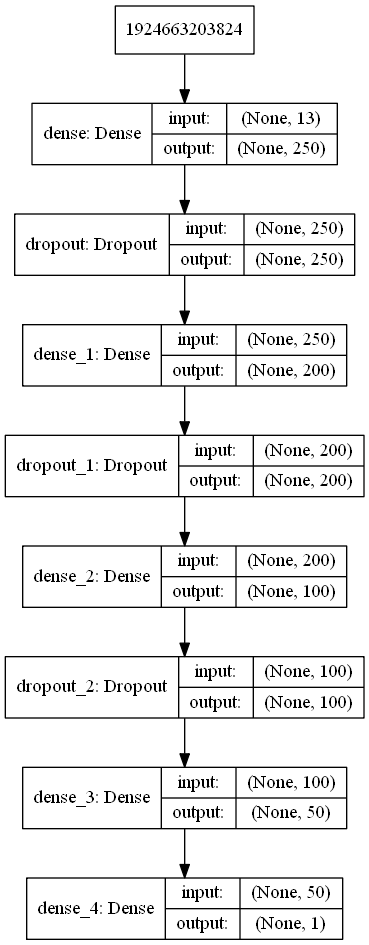
\includegraphics[scale=0.6]{imgs/model_plot.png}
	\caption{Architecture du modèle employé pour le problème de classification du boson de Higgs. L'entrée est un vecteur à 13 paramètres. La structure principale est consitituée de 5 couches internes de types <<dense>>, c'est-à-dire qu'il s'agit de couches possédant des neurones complètement connectés. On ajoute aussi 3 couches de types <<dropout>>, qui viennent atténuer une fraction du signal au hasard lors de la propagation avant. Cette opération tend à réduire le overfitting en forçant le réseau à demeurer versatile. La fraction du signal qui est supprimé par chaque couche dropout est de 0.4, 0.3 et 0.3 respectivement.}
	\label{fig:model}
\end{figure}

\begin{figure}[H]
	\centering
	\begin{subfigure}{.48\textwidth}
		\centering
		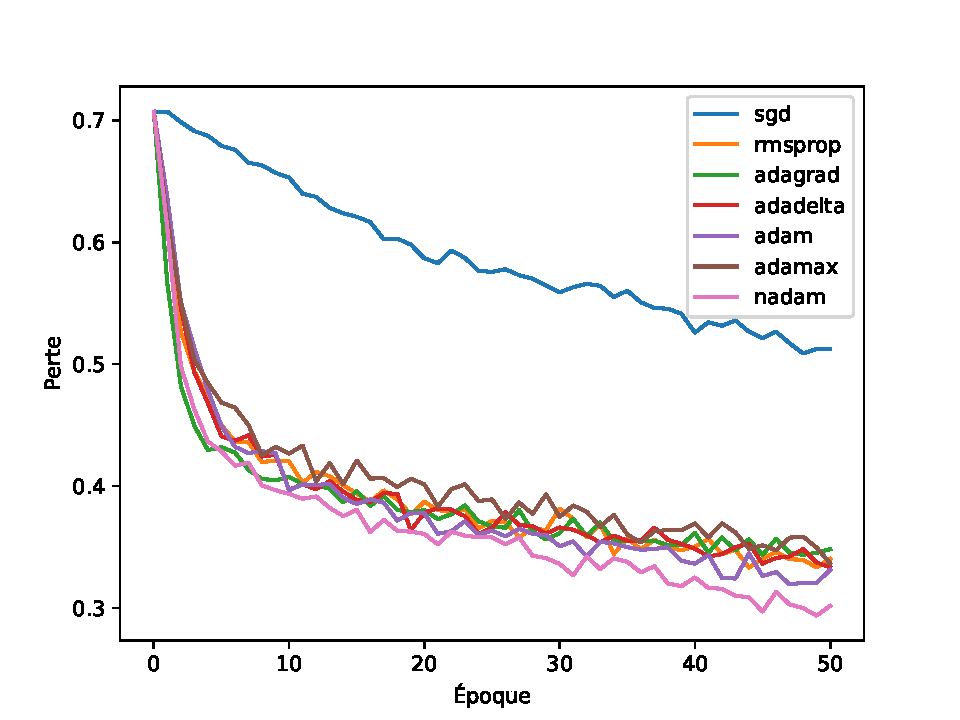
\includegraphics[scale=0.42]{imgs/compare_loss.pdf}
		\caption{La perte sur l'ensemble d'entraînement en fonction de l'époque pour 7 optimiseurs différents.}
	\end{subfigure}
	\hspace{0.2cm}
	\begin{subfigure}{.48\textwidth}
		\centering
		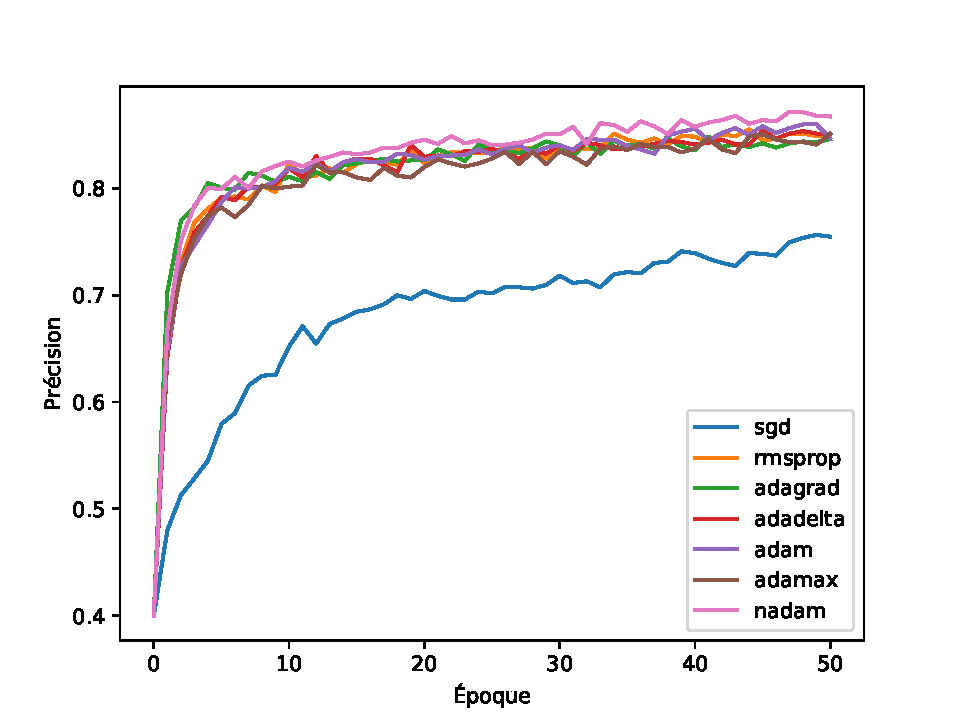
\includegraphics[scale=0.42]{imgs/compare_train_acc.pdf}
		\caption{La précision sur l'ensemble d'entrainement en fonction de l'époque pour 7 optimiseurs différents.}
	\end{subfigure}
	\begin{subfigure}{.48\textwidth}
		\centering
		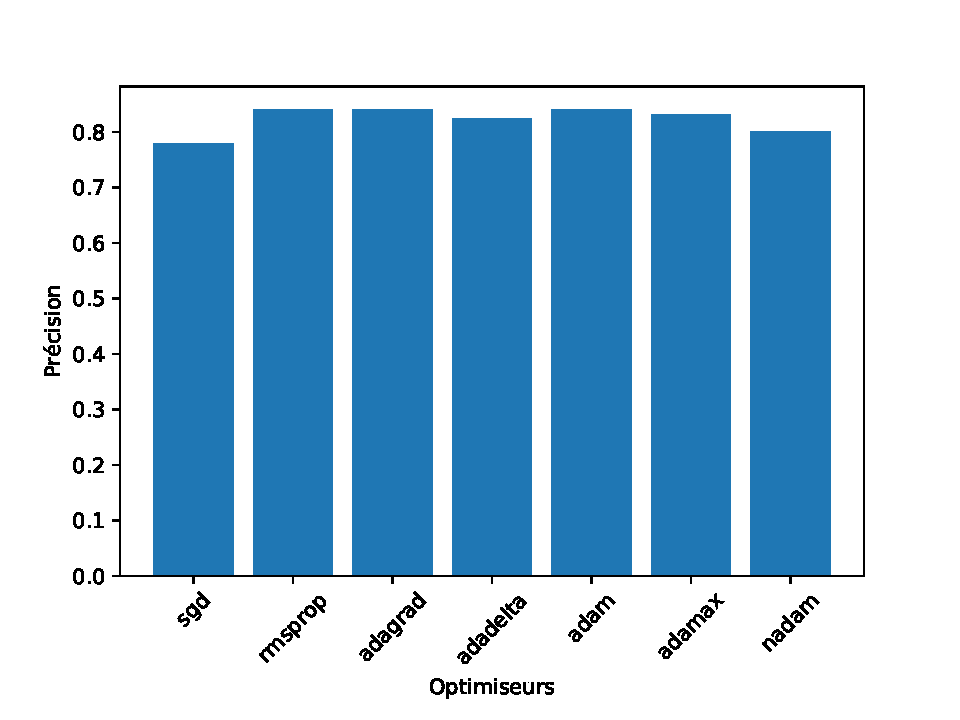
\includegraphics[scale=0.42]{imgs/compare_test_acc.pdf}
		\caption{Précision finale de chaque optimiseur sur l'ensemble test suite à 50 époques d'entraînement.}
	\end{subfigure}
	\caption{Comparaison des optimiseurs offerts par l'interface Keras}
	\label{fig:comp_opti}
\end{figure}

\begin{figure}[H]
	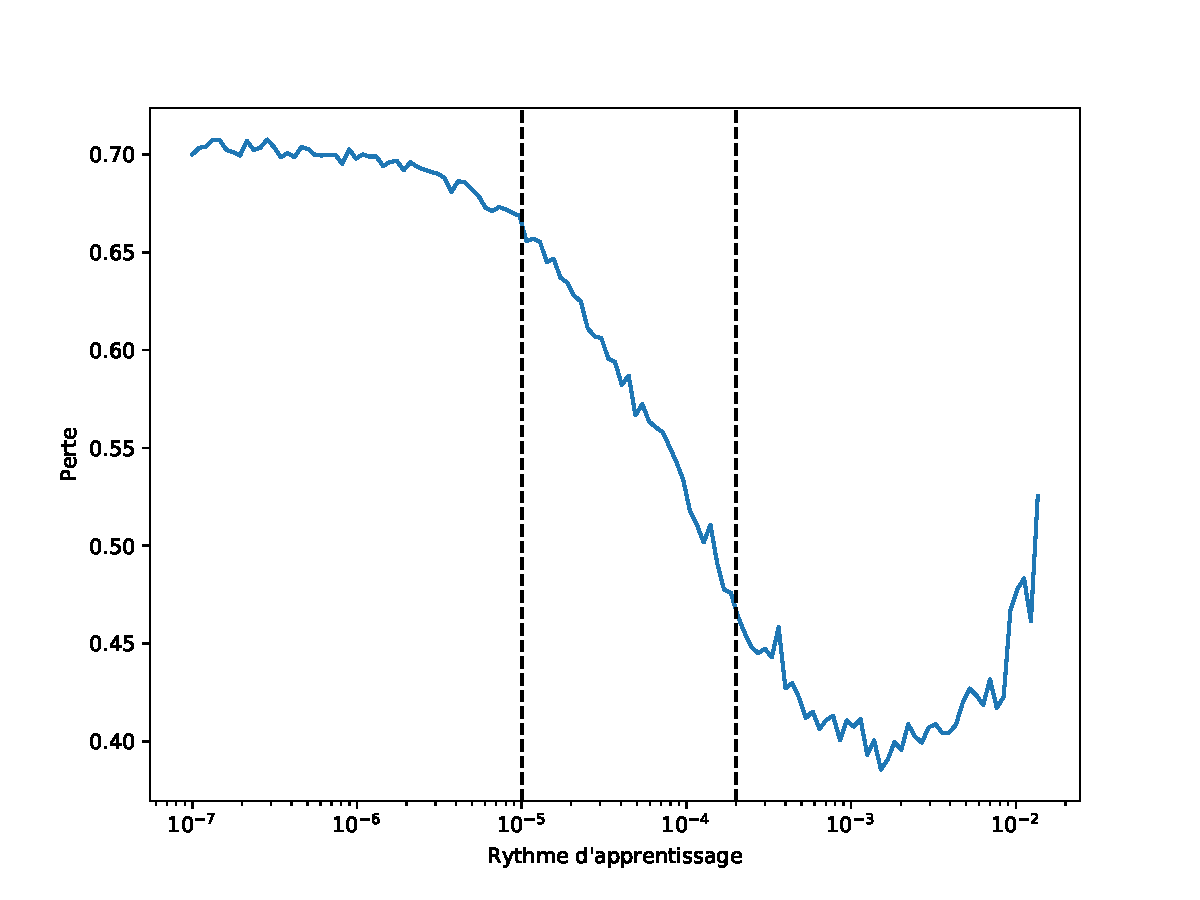
\includegraphics[scale=0.8]{imgs/acc_lr.pdf}
	\caption{Trajectoire d'un entraînement de 125 époques dans l'espace Perte-Rythme d'apprentissage. On débute l'entraînement avec un rythme faible qui évolue selon l'équation \ref{eq:lr} et on mesure la perte à chaque époque. La zone délimitée par les deux barres verticales représente l'intervalle cible pour un rythme d'apprentissage idéal.}
	\label{fig:acc_lr}
\end{figure}


\begin{figure}[H]
	\centering
	\begin{subfigure}{.8\textwidth}
		\centering
		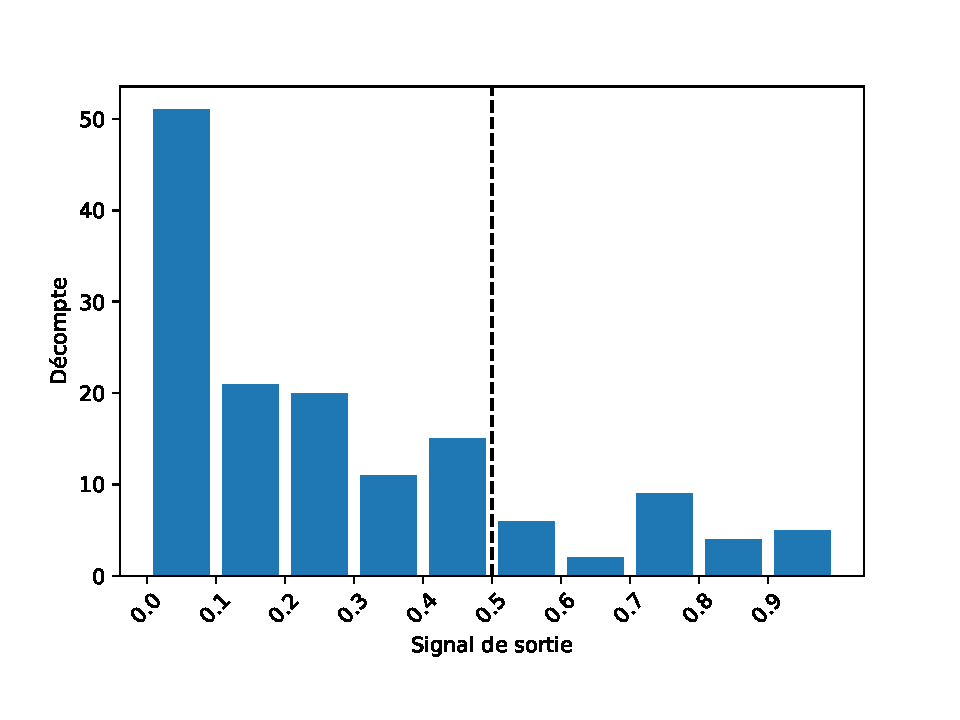
\includegraphics[scale=0.45]{imgs/neg_distri.pdf}
		\caption{Dispersion du signal pour le cas d'un vrai négatif}
	\end{subfigure}
	\begin{subfigure}{.8\textwidth}
		\centering
		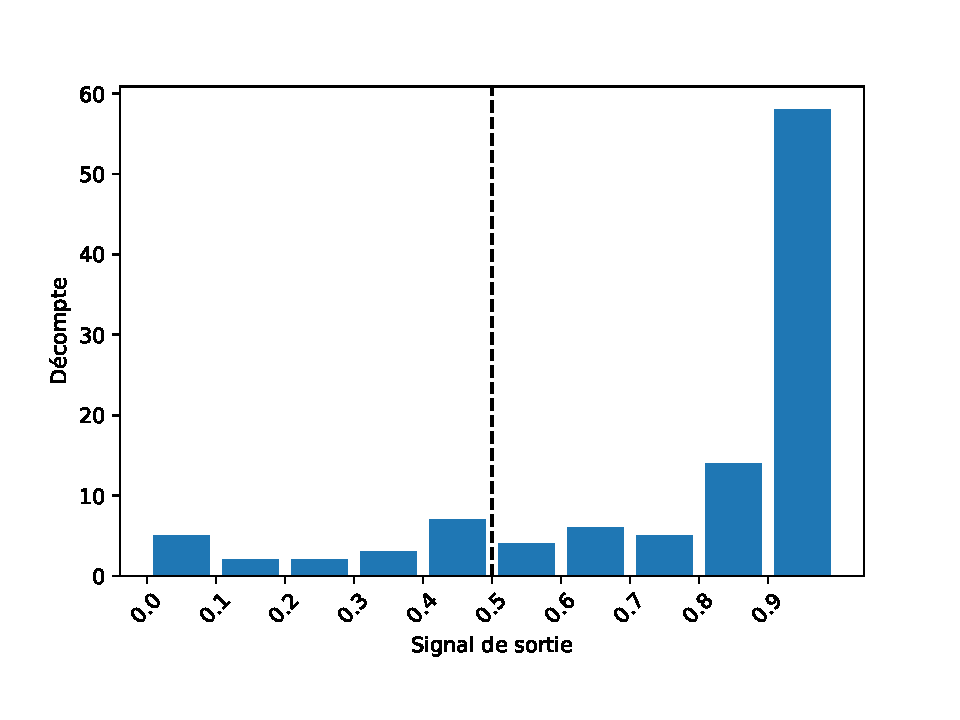
\includegraphics[scale=0.45]{imgs/pos_distri.pdf}
		\caption{Dispersion du signal pour le cas d'un vrai positif}
	\end{subfigure}
	\caption{Dispersion moyenne du signal de sortie sur l'ensemble test pour les 135 réseaux neuronaux employés lors de la classification. La barre verticale sépare les prédictions valides des prédictions erronées.}
	\label{fig:dispersion_signal}
\end{figure}

\section{Bibliographie}\label{sec:bibliographie}
\begin{thebibliography}{l}
	\bibitem{notes_cours} 
	\textsc{Charbonneau}, P., Recueil de notes, Modélisation numérique en physique, Département de Physique, Université de Montréal, Janvier 2019
	
	\bibitem{diro}
	\textsc{Charbonneau}, P., Site web du cours PHY3075, \\ http://www.astro.umontreal.ca/~paulchar/phy3075/phy3075.html
	
	\bibitem{github}
	\textsc{Pfleiderer}, E., Dépôt GitHub,\\ https://github.com/EricPfleiderer/Portfolio/tree/master/PHY3075/PROJET6
	
	\bibitem{tensorflow}
	\textsc{Tensorflow}, Librairie à code source ouvert d'apprentissage machine,\\
	www.tensorflow.org
	
	\bibitem{keras}
	\textsc{Keras}, Interface de programmation d'apprentissage machine,\\
	www.keras.io
	
\end{thebibliography}


\end{document}